\cleardoublepage

\chapter{Analiza wyników badania}
W niniejszym rozdziale autor zaprezentował analizę stworzonych systemów RAG pod kątem dokładności, liczby zużytych tokenów, czasu oraz przepustowości podczas generowania odpowiedzi. Warto nadmienić, iż na wykresach kolorem niebieskim oznaczono rezultaty dla systemów RAG zawierających dane nieustrukturyzowane, a czerwonym rezultaty dla systemów RAG zawierających dane ustrukturyzowane.

    
    \section{ Dokładność odpowiedzi }
    W celu zmierzenia dokładności odpowiedzi dużych modeli językowych w systemach RAG, autor pracy oceniał odpowiedzi zero-jedynkowo. Jeżeli odpowiedź była poprawna — trafnie odpowiadała na zadane pytanie — uznawana była za pozytywną (1), a w przeciwnym razie za negatywną (0). Warto podkreślić, że odpowiedzi nie były deterministyczne. Na poniższym rysunku \ref{dokladnosc_wyniki} przedstawiono wykres dokładności w procentach dla konkretnej konfiguracji systemu RAG.

    \begin{center}
        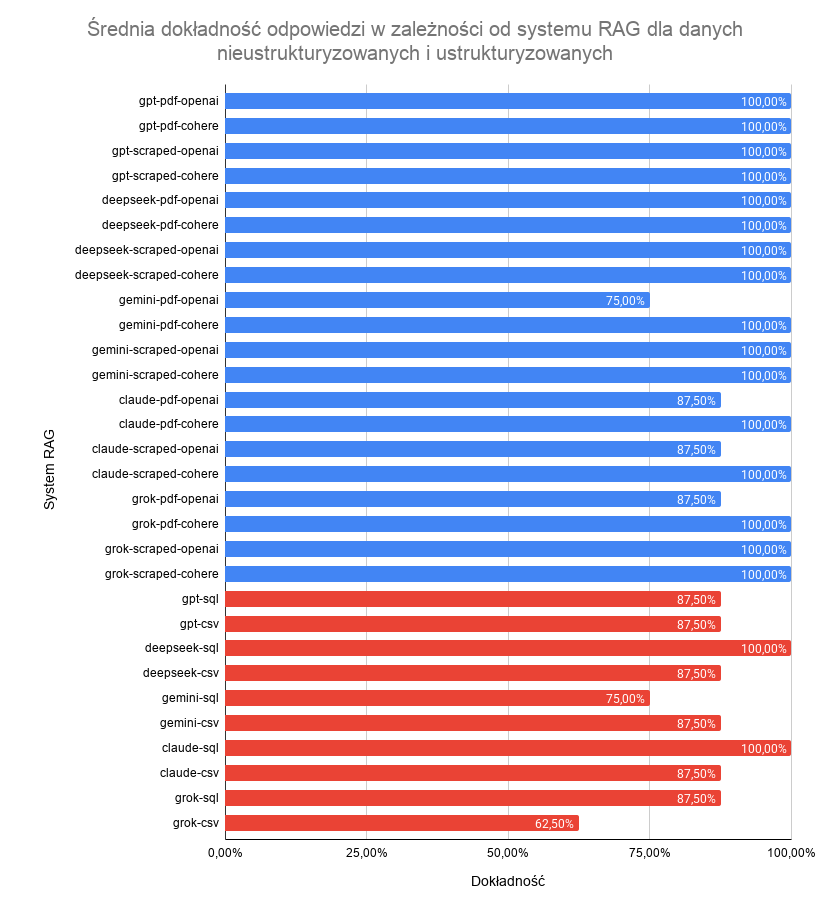
\includegraphics[width=0.8\textwidth]{rysunki/dokladnosc_wyniki.png}
        \captionof{figure}{ Średnia dokładność wygenerowanej odpowiedzi w zależności od systemu RAG dla danych nieustrukturyzowanych i ustrukturyzowanych }
        \label{dokladnosc_wyniki}
    \end{center}

    Zaobserwowano, że badane modele wykazały wysoką zdolność do udzielania poprawnych odpowiedzi na zadane pytania. Aż 18 na 30 konfiguracji RAG poradziło sobie bezbłędnie. Odnosząc się do danych nieustrukturyzowanych, LLMy znacznie lepiej poradziły sobie z interpretacją pliku tekstowego (scraped) niż PDF. Natomiast, w odniesieniu do danych ustrukturyzowanych, odpowiedzi dotyczące pliku SQL były trafniejsze niż te dotyczące pliku CSV. Zdecydowanie lepiej poradziły sobie LLMy przeznaczone do odpowiadania na pytania w oparciu o dane nieustrukturyzowane. Model deepseek-v3.2-exp wyróżnił się największą dokładnością i pomylił się łącznie tylko w jednym pytaniu. W kwestii embeddera, znacznie lepiej poradził sobie model od firmy Cohere niż OpenAI. Systemy RAG wykorzystujące ten embedder wykazały się 100\% skutecznością. Najgorzej wypadła konfiguracja grok-csv, w której model odpowiedział dobrze tylko na pięć z ośmiu pytań (62,50\%). Co ciekawe, drugie pytanie z kategorii integracji informacji okazało się najcięższe dla dużych modeli językowych w ramach nieustrukturyzowanego dokumentu. W czterech odpowiedziach z dwudziestu  padło stwierdzenie, że informacja o liczbie parametrów modelu GPT-1 nie została zawarta w tekście. Z kolei, w ramach pliku CSV, modele nie umiały odpowiedzieć na drugie średniozaawansowane pytanie, gdyż pojawiał się błąd: \enquote{'Price > 920' nie jest liczbą}.


    \section{ Zużycie tokenów }
    W drugim kroku, przeanalizowano koszty — liczbę tokenów zużytych przez modele do interpretacji zapytania i wygenerowania odpowiedzi. Na rysunku \ref{tokeny_wyniki} przedstawiono rezultaty testu.

    \begin{center}
        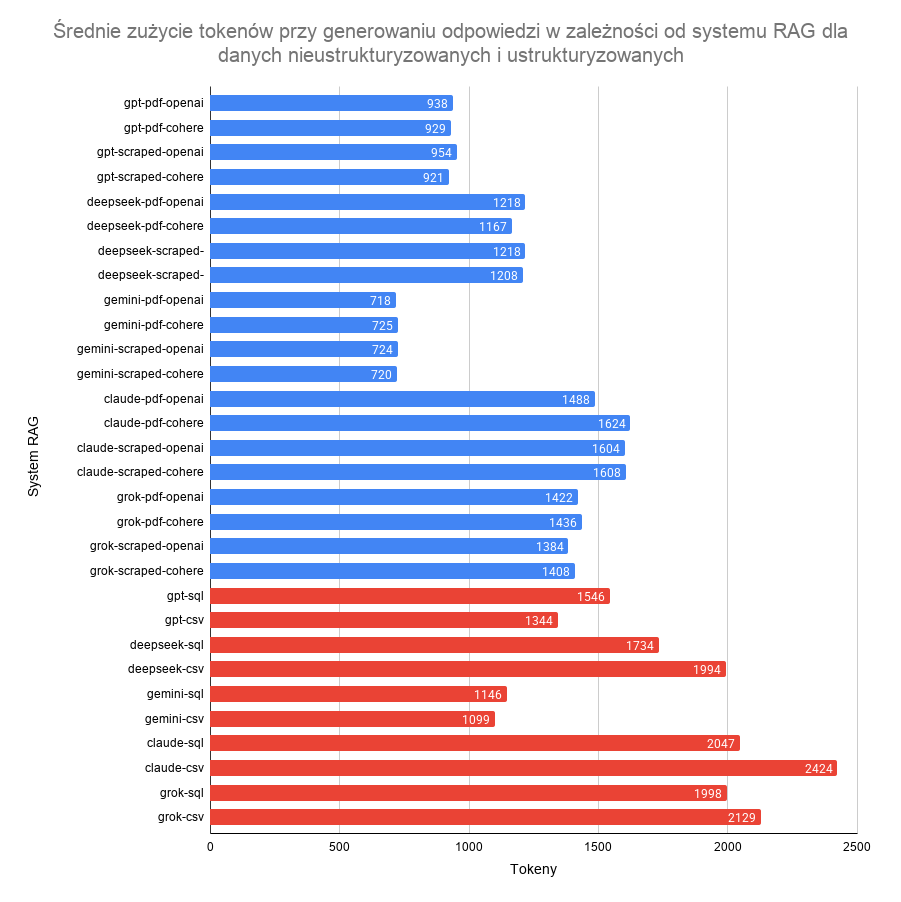
\includegraphics[width=0.88\textwidth]{rysunki/tokeny_wyniki.png}
        \captionof{figure}{ Średnie zużycie tokenów podczas generowania odpowiedzi w zależności od systemu RAG dla danych nieustrukturyzowanych i ustrukturyzowanych }
        \label{tokeny_wyniki}
    \end{center}

    Uzyskane wyniki wskazują, iż znacznie bardziej kosztowne jest stosowanie systemu RAG z danymi ustrukturyzowanymi (średnie zużycie: 1746 tokenów) niż nieustrukturyzowanymi (średnie zużycie: 1171 tokenów). Dla obu rodzajów danych trudno jest jednoznacznie stwierdzić, w ramach których dokumentów wygenerowanie odpowiedzi było najmniej kosztowne. Podobna sytuacja ma miejsce przy określaniu najbardziej wydajnego modelu embeddingowego. Łatwo dostrzec, że systemy stosujące gemini-3-flash-preview wypadają najkorzystniej, ponieważ średnie zużycie wyniosło tylko 855 tokenów. Przeciwieństwo stanowi claude-haiku-4.5, który średnio zużył ponad dwa razy więcej tokenów, aż 1799.
    
    
    \section{ Czas generowania odpowiedzi }
    W kolejnym kroku, porównano systemy RAG pod kątem czasu generowania odpowiedzi. Poniższy rysunek \ref{czas_wyniki} prezentuje te rezultaty.
    
    \begin{center}
        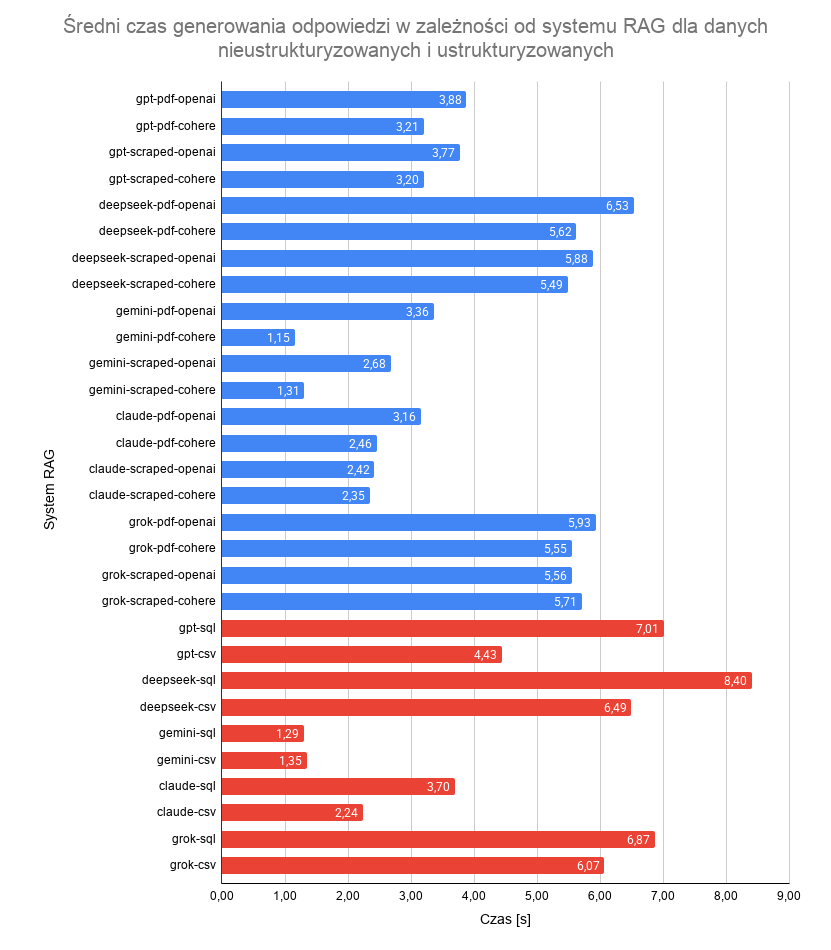
\includegraphics[width=0.8\textwidth]{rysunki/czas_wyniki.png}
        \captionof{figure}{ Średni czas potrzebny na wygenerowanie odpowiedzi w zależności od systemu RAG dla danych nieustrukturyzowanych i ustrukturyzowanych }
        \label{czas_wyniki}
    \end{center}

    Z wykresu wynika, iż znacznie mniej czasochłonne jest wygenerowanie odpowiedzi dla systemów RAG zawierających dane nieustrukturyzowane (średni czas: 3,96 sekund) niż ustrukturyzowane (średni czas: 4,78 sekund). Dla pierwszego rodzaju danych łatwo zauważyć, że odpowiedzi w ramach pliku CSV generowane są znacznie szybciej. Powodem może być fakt hostowania pliku na tej samej platformie, na której było przeprowadzone badanie. Dla drugiego rodzaju danych można zauważyć, że odpowiedzi w ramach pliku tekstowego (scraped) są generowane szybciej. Może to wynikać z jego prostej struktury, charakterystycznej dla plików markdown. Co ciekawe, systemy RAG stosujące embedder od OpenAI są znacznie wolniejsze od analogicznych systemów wykorzystujących embedder od Cohere. Najszybszym modelem okazał się być model gemini-3-flash-preview (średni czas: 1,86 sekund), a najwolniejszym deepseek-v3.2-exp (średni czas: 6,40 sekund).
    
    
    \section{ Przepustowość tokenów }
    W ostatnim kroku, przeanalizowano systemy RAG pod kątem przepustowości tokenów — liczby zużytych tokenów na sekundę — podczas generowania odpowiedzi. Posiadając wyniki z dwóch poprzednich podrozdziałów, można było w łatwy sposób obliczyć przepustowość ze wzoru \ref{wzór_przepustowość_odpowiedzi_llm}. Na poniższym rysunku \ref{przepustowosc_wyniki} zobrazowano wyniki tych obliczeń.
    
    \begin{center}
        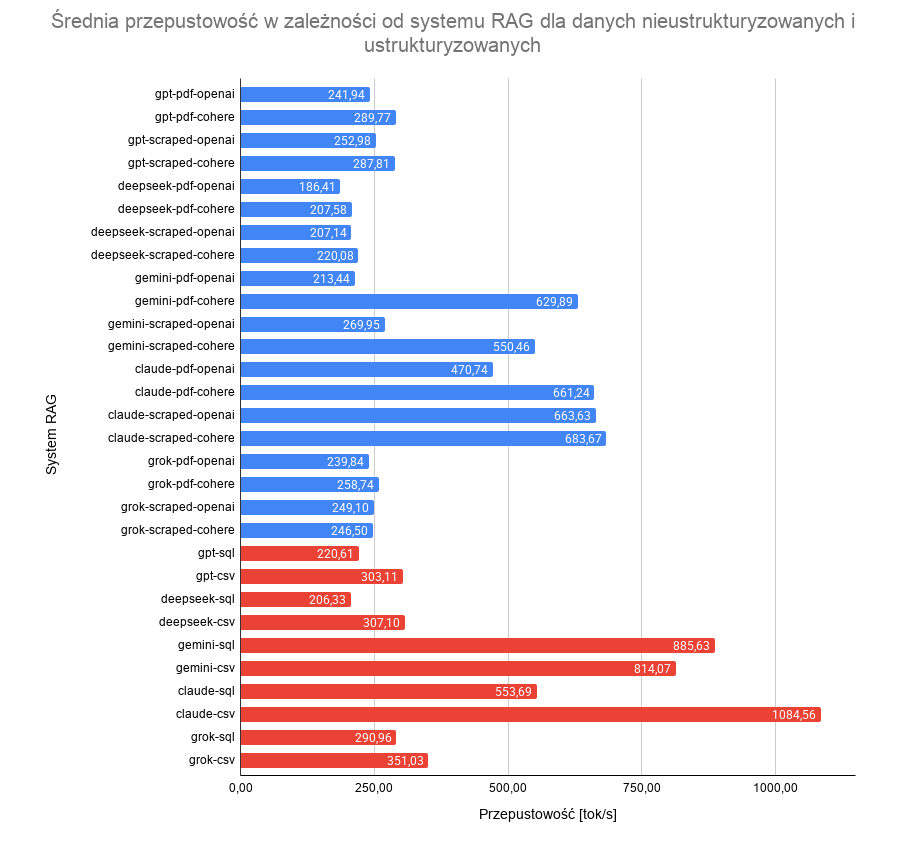
\includegraphics[width=0.9\textwidth]{rysunki/przepustowosc_wyniki.png}
        \captionof{figure}{ Średnia przepustowość w zależności od systemu RAG dla danych nieustrukturyzowanych i ustrukturyzowanych }
        \label{przepustowosc_wyniki}
    \end{center}
    
    Z wykresu wynika, że w przyjętym scenariuszu testowym znacznie większą przepustowością charakteryzują się systemy RAG zawierające dane ustrukturyzowane (średnio 501,71 tok/s) niż te zawierające dane nieustrukturyzowane (średnio 351,54 tok/s). Można zauważyć, że przepustowość była znacznie wyższa dla systemów zawierających plik CSV niż bazę SQL. Dla danych nieustrukturyzowanych dostrzeżono, iż systemy z plikiem tekstowym (scraped) mają niewiele większą przepustowość tokenów (średnio o 23 tok/s) niż te z plikiem PDF. Z wykresu i obliczeń jasno wynika, że embedder od Cohere charakteryzuje się lepszymi wynikami niż embedder od OpenAI w każdej konfiguracji RAG w tym teście. Optymalnym dużym modelem językowym okazał się być claude-haiku-4.5, gdyż średnia przepustowość w związanych z nim systemach wyniosła 686,26 tok/s.
    

    \section{ Wnioski }
    Zaprezentowane przez autora wyniki nie są porównywalne z rezultatami zaprezentowanymi w artykułach \cite{art2_unstructured2024} i \cite{art3_structured2024}. Warto mieć na uwadze, że z racji na ograniczenia czasowe testy wykonywane przez autora pracy dyplomowej zostały przeprowadzone dla każdego rodzaju danych za pomocą tylko ośmiu a nie kilkuset czy nawet kilku tysięcy zróżnicowanych pytań.
    
    Wybrano dwie optymalne konfiguracje RAG spośród badanych. W ramach nieustrukturyzowanych dokumentów za najlepszy system uznano gpt-scraped-cohere. Wyróżnił się stuprocentową dokładnością i generował stosunkowo mało tokenów w krótkim czasie. Natomiast, w ramach danych ustrukturyzowanych za najlepszy system uznano claude-sql. Pomimo zużycia największej liczby tokenów, także zapewnił stuprocentową skuteczność odpowiedzi bardzo szybko odpowiadając na zadane pytania.
        
    
    \section{ Implementacja optymalnego rozwiązania z wykorzystaniem graficznego interfejsu użytkownika }

    Oba systemy RAG, które w poprzednim podrozdziale zostały wybrane za najwydajniejsze spośród badanych konfiguracji, udostępniono za pomocą graficznego interfejsu użytkownika. Stronę wykonano za pomocą narzędzia Lovable \cite{lovable}, a hosting odbywa się lokalnie. Na poniższym rysunku \ref{gui_lovable} przedstawiono GUI wraz z przykładową konwersacją.
    
    \begin{center}
        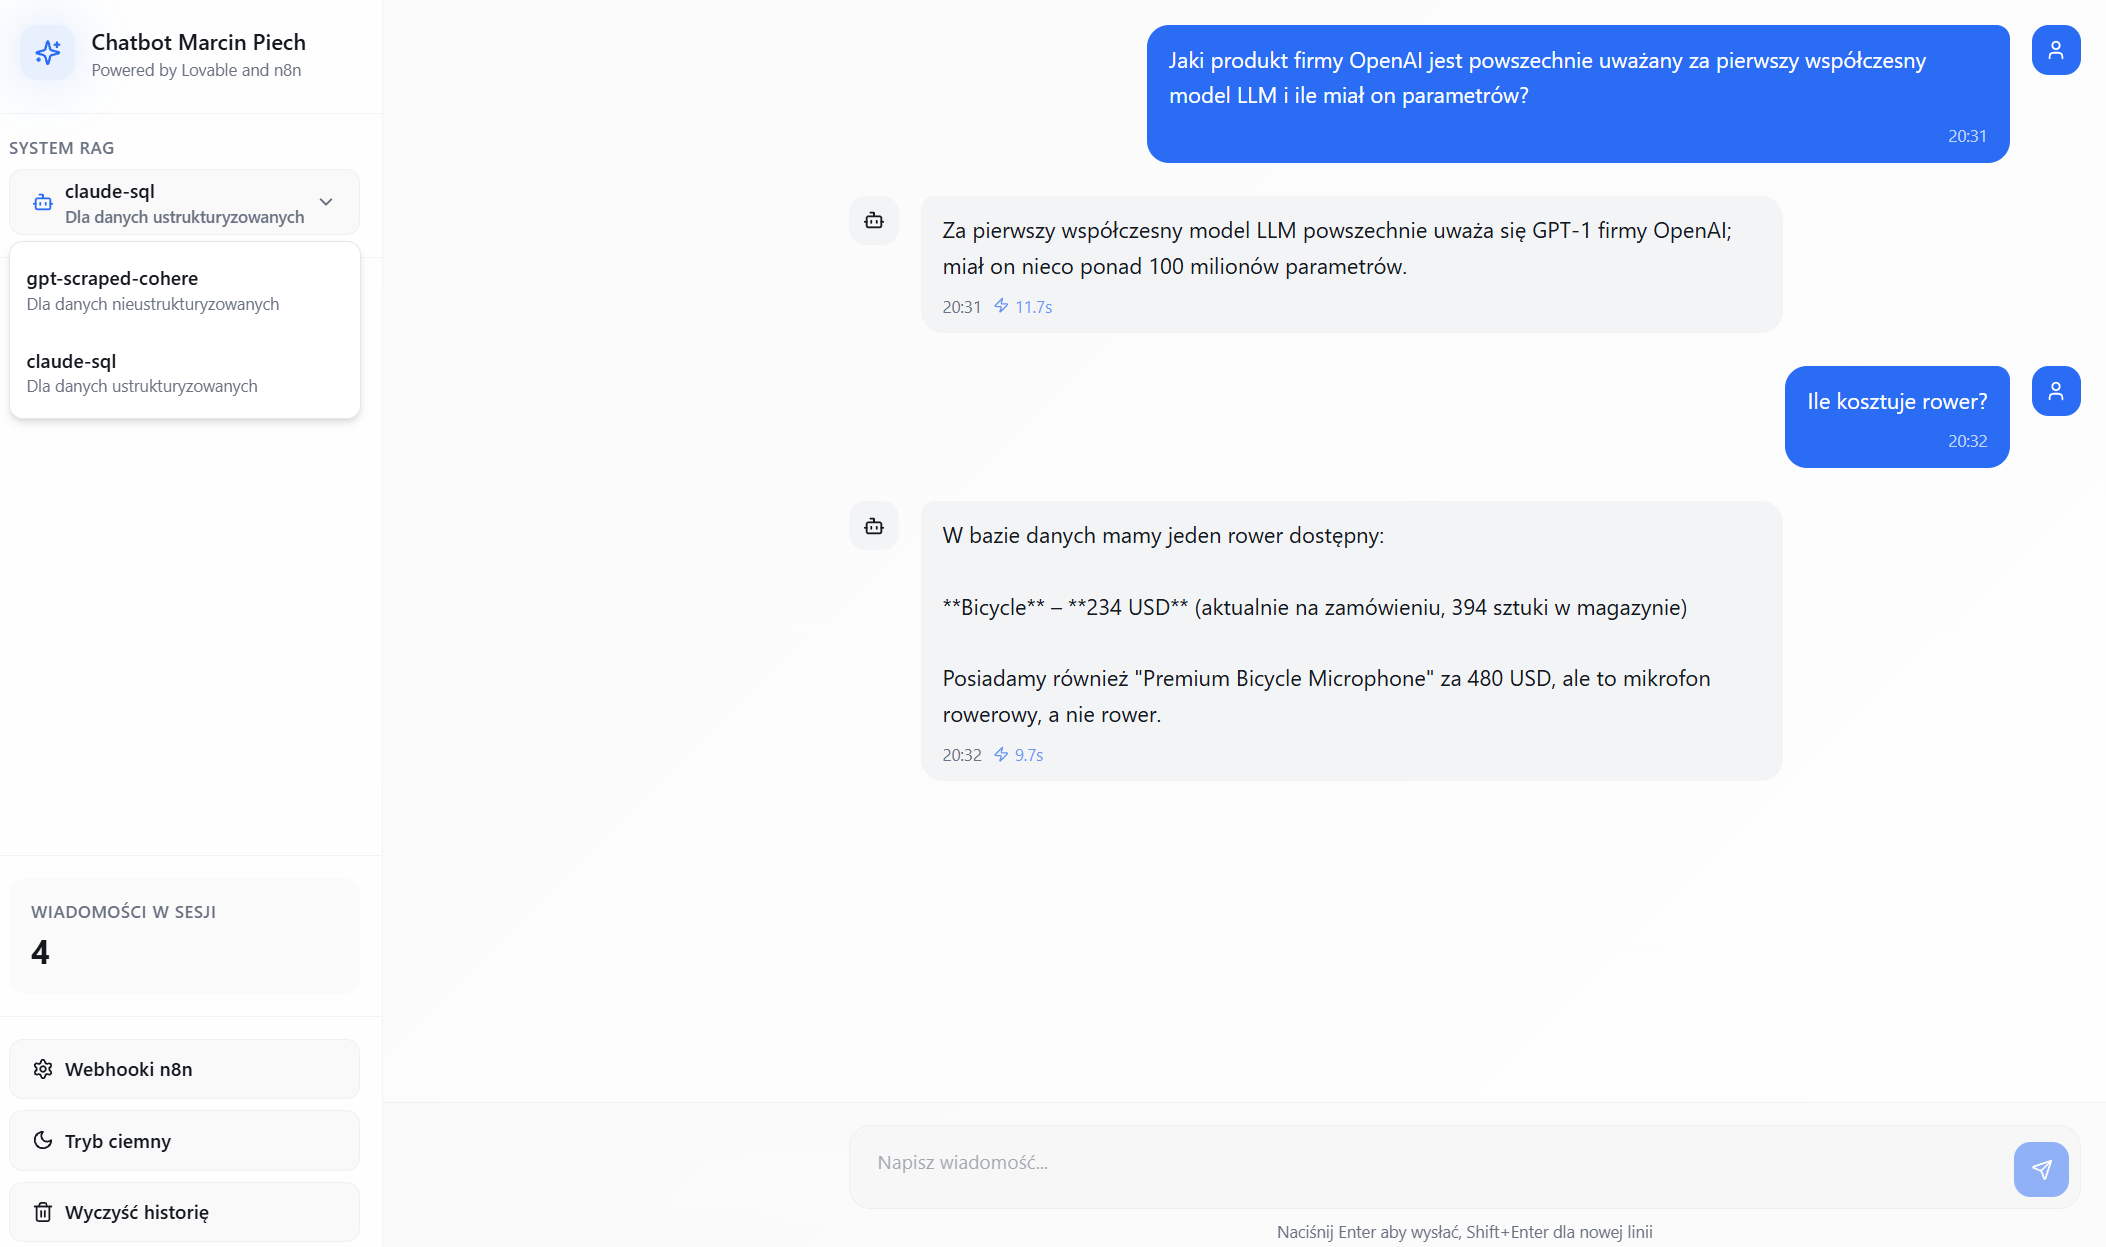
\includegraphics[width=0.9\textwidth]{rysunki/gui_lovable.png}
        \captionof{figure}{ Graficzny interfejs użytkownika służący do implementacji dwóch najwydajniejszych konfiguracji RAG dla danych nieustrukturyzowanych i ustrukturyzowanych \cite{lovable}}
        \label{gui_lovable}
    \end{center}
    
    \noindent Dostępna jest możliwość wyboru systemu RAG, na bazie którego chce się prowadzić konwersację — gpt-scraped-cohere lub claude-sql. Co ciekawe, w ramach jednej konwersacji można prowadzić dialog z dwoma systemami. Na załączonym obrazie \ref{lovable_webhooki_n8n} widnieje tego przykład. Pierwsza wiadomość została wysłana do gpt-scraped-cohere a druga do claude-sql. W lewym dolnym rogu widnieje liczba wiadomości w obecnej sesji, przycisk do zmiany motywu na ciemny oraz przycisk do wyczyszczenia konwersacji (rozpoczęcia dialogu od nowa). Znajdziemy tam także przycisk do konfiguracji adresów URL webhooków z dedykowanego workflow w n8n, które umożliwiają połączenie backendu (program w n8n) z frontendem (interfejs użytkownika).

    \begin{center}
        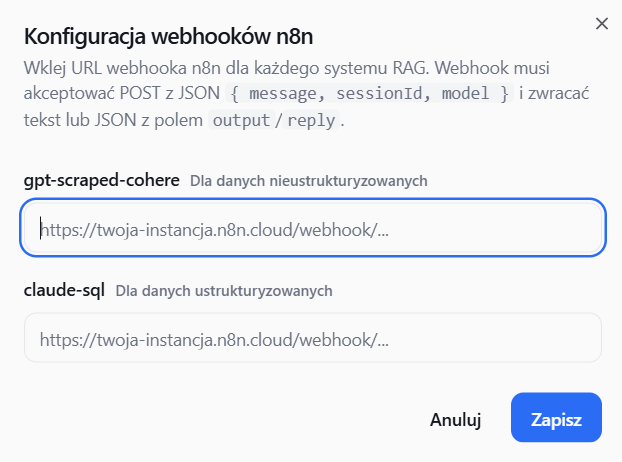
\includegraphics[width=0.45\textwidth]{rysunki/lovable_webhooki_n8n.png}
        \captionof{figure}{ Widok okna służącego do konfiguracji adresów URL webhooków w n8n dedykowanych dla konkretnych systemów RAG \cite{lovable}}
        \label{lovable_webhooki_n8n}
    \end{center}
    
    \noindent Warto zauważyć, że każda z odpowiedzi chatbota zawiera informację o której godzinie została dostarczona i ile czasu zajęło jej wygenerowanie w sekundach. 

    Konwersacja z dwoma dużymi modelami językowymi może się odbywać dzięki wcześniej wspomnianemu oprogramowaniu w n8n. Na poniższym rysunku \ref{mgr_gui_n8n} przedstawiono dwa procesy przetwarzania zapytania. Workflow po lewej stronie, zaczynające się od węzła Webhook1, odzwierciedla wybrany system RAG przeznaczony do danych nieustrukturyzowanych (gpt-scraped-cohere). Workflow po prawej stronie, zaczynający się od węzła Webhook2, reprezentuje wybrany system RAG przeznaczony do danych ustrukturyzowanych (claude-sql).
    
    \begin{center}
        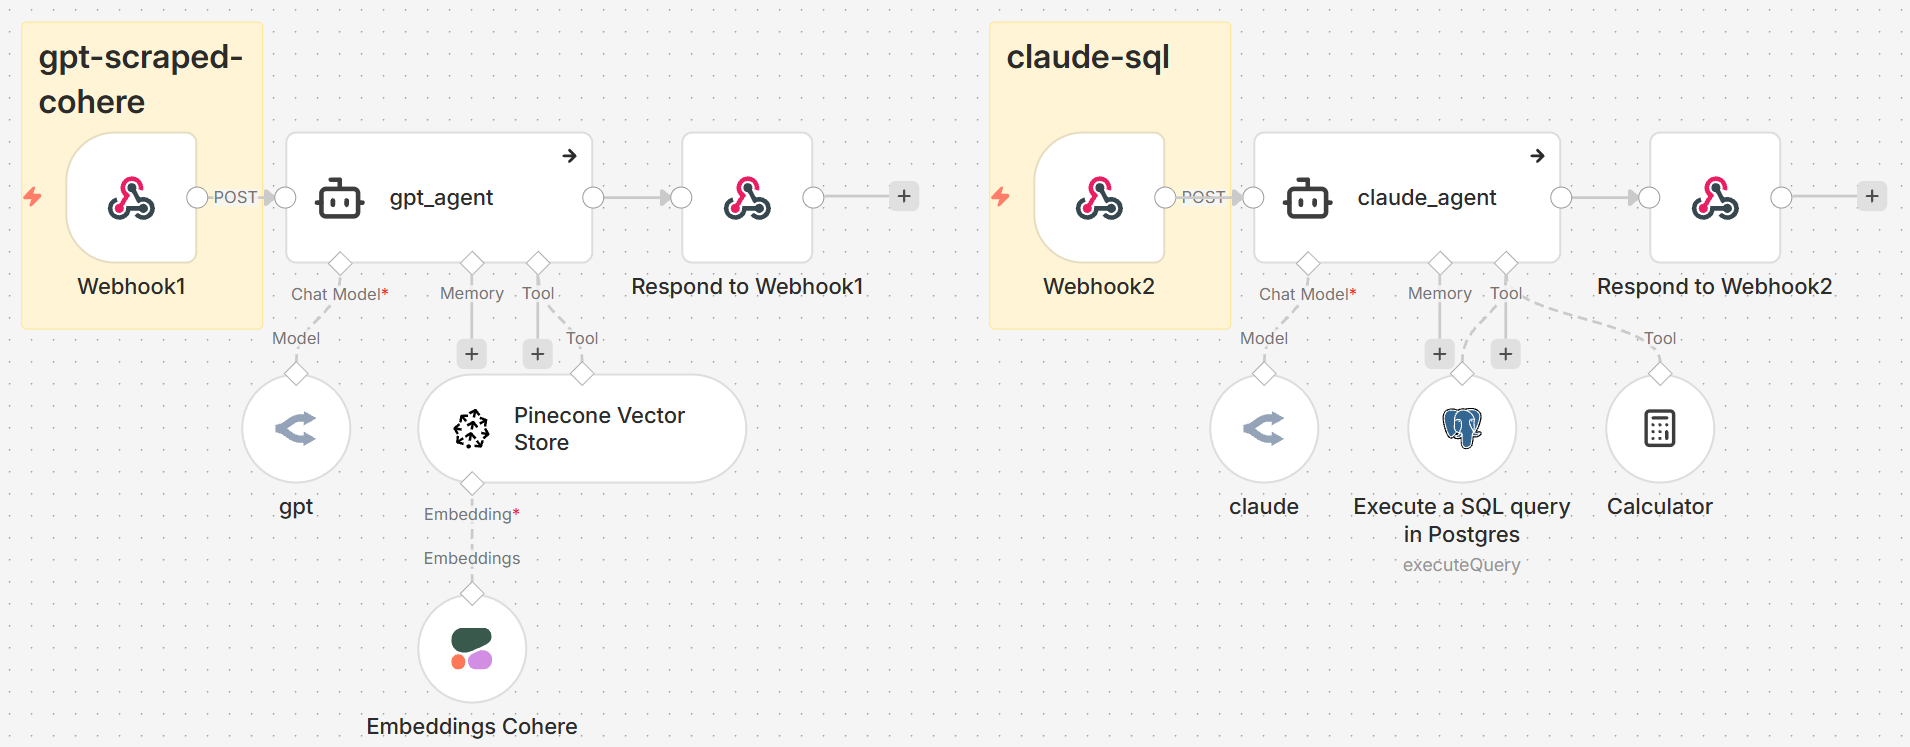
\includegraphics[width=0.9\textwidth]{rysunki/mgr_gui_n8n.png}
        \captionof{figure}{ Oprogramowanie w n8n służące do konwersacji z dwoma najwydajniejszymi konfiguracjami RAG za pomocą graficznego interfejsu użytkownika \cite{n8n}}
        \label{mgr_gui_n8n}
    \end{center}

    Węzły Webhook1 i Webhook2 są ustawione w stan aktywnego nasłuchiwania (published). Warto dodać, iż są one ustawione na odbieranie żądań HTTP metodą POST. Dzięki temu pytanie zadane przez użytkownika poprzez GUI zostaje przekazane w czasie rzeczywistym do konkretnego agenta AI. Następnie, wygenerowana odpowiedź trafia do odpowiedniego węzła Respond to Webhook. Pozwala on przekazać tę wiadomość do GUI, co umożliwia zachowanie ciągłości konwersacji i kolejności wiadomości.